% !TeX root = ../Main-Report.tex

\chapter{Simscape Multibody Modeling}

The Multibody model of the robot has been created using the \textsc{Simscape Multibody Link Plugin} and several files that have been given by the lecturer. Using the plugin, it is possible to create a simulation from an exported .xml file and several .step-files, both exported from CAD-software, in this case from \textsc{Solidworks}. The resulting model has then been slightly adjusted to be usable for the tasks at hand. These adjustments include:

\begin{itemize}
	\item the addition of a transform sensor, which is able to measure the relative transform between the origin of our chosen coordinate system and the end-effector.
	\item the addition of several transform adjustments, to ensure the correct detection of the relative transform.
	\item the addition of position input ports to the prismatic joints, to be able to control them accordingly.
	\item the addition of three subsystems, which automatically compute the first two derivatives of the input position information and perform a sign-correction.
\end{itemize}

A screenshot of how the adjusted model looks can be seen in figure \ref{fig:mbmodeldelta}.

\begin{figure}[H]
	\centering
	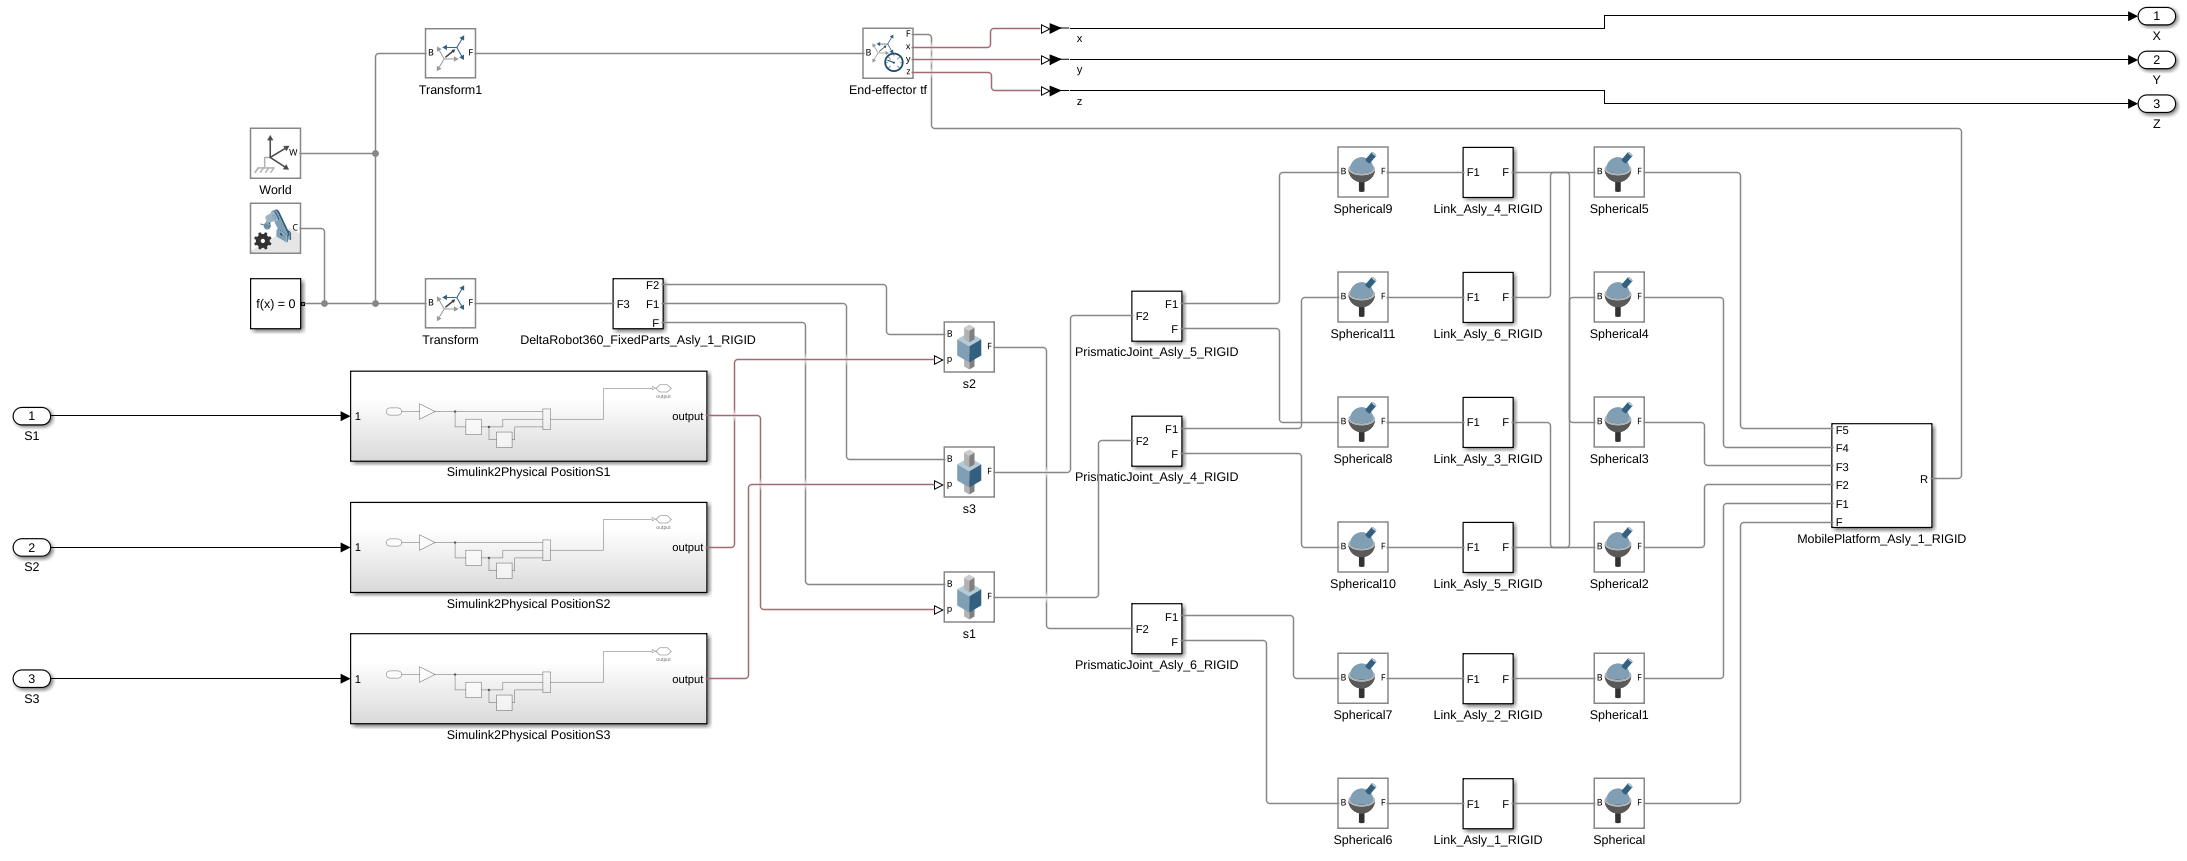
\includegraphics[width=1.0\linewidth]{cus_imgs/MB_model_delta}
	\caption{Adjusted Simscape Multibody model of the robot}
	\label{fig:mbmodeldelta}
\end{figure}
